\documentclass[conference]{IEEEtran}
\IEEEoverridecommandlockouts
\usepackage{graphicx}
\usepackage{url}

\providecommand{\toprule}{\hline\hline}
\providecommand{\midrule}{\hline}
\providecommand{\bottomrule}{\hline\hline}
\providecommand{\text}[1]{\mbox{#1}}
\renewcommand{\texttt}[1]{\textsf{#1}}

\def\BibTeX{{\rm B\kern-.05em{\sc i\kern-.025em b}\kern-.08em
    T\kern-.1667em\lower.7ex\hbox{E}\kern-.125emX}}

\begin{document}

\title{A Context-Aware Hybrid Reinforcement Learning Framework for CPU Scheduling in Virtualized Systems}

\author{\IEEEauthorblockN{Shri Shailesh (24BDS0415), Sriram (24BCE2695), Sahasrad (24BDS0405)}
\IEEEauthorblockA{\textit{School of Computer Science and Engineering, VIT Vellore} \\
Vellore, Tamil Nadu, India}
}

\maketitle

\begin{abstract}
Hardware consolidation via lightweight virtualization enables concurrent virtual machines (VMs) to execute across resource-constrained edge platforms. However, static dispatching heuristics struggle to maintain quality of service under highly dynamic, unpredictable workload regimes. This paper proposes a context-aware hybrid reinforcement learning scheduling framework designed to overcome the myopic nature of classical heuristics and pure bandit policies. The proposed Hybrid policy augments a linear Contextual Bandit Reinforcement Learning (CB-RL) core with an online moving-average workload demand predictor, dynamic starvation-free priority adjustment, a normalized estimated energy penalty term, density-aware completion hysteresis, and a bounded first-touch responsiveness boost. We conduct a rigorous comparative evaluation against Priority-Based Round Robin (PRR), Priority-Based Monotonic (PRM), and standalone CB-RL across 1,500 deterministic simulation runs spanning diverse VM densities, workload profiles, and simulated processor architectures (ARM-like, x86-like, and RISC-V-like). On the x86-like reference configuration, the measured Hyper-Optimized Hybrid policy records \textbf{228.55} ticks waiting time, \textbf{249.09} ticks turnaround time, and \textbf{132.46} ticks response time; the response result is a 51.4\% reduction relative to PRM, with a measured deadline-miss rate of \textbf{0.5561}.
\end{abstract}

\begin{IEEEkeywords}
Lightweight virtualization, CPU scheduling, contextual bandit, reinforcement learning, workload prediction, dynamic priority, energy-aware systems.
\end{IEEEkeywords}

\section{Introduction}
Modern embedded edge computing and Internet of Things (IoT) ecosystems increasingly leverage lightweight virtualization hypervisors (such as Xvisor) to achieve robust software isolation and efficient resource sharing on compact microprocessors. In these shared-processor environments, the underlying virtual CPU (vCPU) scheduling policy represents a pivotal operational component dictating overall throughput, deadline compliance, and latency guarantees.

Conventional virtualization schedulers rely predominantly on rigid, deterministic rules such as Priority-Based Round Robin (PRR) or period-centric Priority-Based Monotonic (PRM) dispatching. Although computationally negligible, these static heuristics exhibit notable performance degradation during abrupt traffic shifts, as their decision logic remains insensitive to transient queue dynamics, task progress, and evolving contention levels. To alleviate these limitations, machine learning algorithms, specifically reinforcement learning (RL), have emerged as a viable paradigm to dynamically condition scheduling selections on real-time system state.

A prominent baseline study by Cui et al. [1] integrated a linear Contextual Bandit (CB-RL) scheduler with virtualized networking mechanisms (RPMsg) on an embedded ARM platform, demonstrating noticeable improvements in scheduling responsiveness. Building upon this foundational premise, the present work isolates, expands, and thoroughly benchmarks the core scheduling logic within a fully reproducible single-core discrete-event simulation framework. Rather than relying on purely reactive bandit policies, we develop an adaptive Hybrid scheduling framework that integrates predictive demand estimation, dynamic priority rejuvenation, completion-margin hysteresis, and energy-conscious regularization to optimize multiprogramming efficiency across diverse virtual machine populations.

\section{Related Work}
Adaptive processor scheduling and intelligent resource management have garnered significant research interest across the systems and artificial intelligence communities. The direct conceptual predecessor of this study is the eXvisor scheduling architecture presented by Cui et al. [1], which utilized contextual bandit formulations to govern virtual core time-slicing on physical hardware.

Beyond contextual bandits, deep reinforcement learning architectures have been explored for fine-grained operating system control. Zhou and Lin [2] deployed deep RL models for real-time Dynamic Voltage and Frequency Scaling (DVFS), demonstrating the capacity of learning agents to navigate complex energy-performance trade-offs in real-time embedded environments. Similarly, Li et al. [3] and Sun et al. [4] investigated Double DQN architectures for dynamic thread scheduling and adaptive operating system task orchestration, highlighting the efficacy of state-space feature representations in capturing queue contention. Complementing learning-driven techniques, Rinku and AshaRani [5] underscored the necessity of continuous priority reassessment to counteract task starvation and priority inversion in multiprogrammed workloads.

In vehicular and mobile edge systems, energy awareness constitutes an equally critical optimization objective. Perin et al. [6] formulated energy-aware scheduling heuristics (EASE) to reconcile computational demands with green energy constraints. Contextualizing these individual advancements, Zhang et al. [7] provided a broad taxonomy of AI-driven operating system designs, arguing that modern OS kernels benefit substantially from hybrid controllers that pair formal algorithmic bounds with lightweight adaptive inference. Motivated by these insights, our research synthesizes these orthogonal paradigms into a coherent, lightweight scheduling mechanism evaluated under strictly controlled architectural settings.

\section{Problem Statement}
In constrained multi-tenant edge virtualization, a single physical execution core must be arbitrated among multiple virtual machines exhibiting heterogeneous arrival distributions, distinct CPU burst demands, and varying deadline criticalities. Under static scheduling regimes such as PRR and PRM, dispatching decisions remain decoupled from transient workload variations. Consequently, systems subjected to bursty or compute-intensive traffic suffer from prolonged task waiting times, elevated deadline miss ratios, and severe degradation in allocation fairness.

The fundamental research inquiry addressed herein is whether an augmented, context-aware reinforcement learning scheduler --- incorporating short-term moving-average workload prediction, continuous priority aging, completion hysteresis, and power-rate regularization --- can attain a superior operational balance compared to both classical heuristic schedulers and unaugmented contextual bandits, and under what specific workload and hardware characteristics these advantages materialize.

\section{Research Gap}
While the contextual bandit scheduler formulated in [1] demonstrates superior responsiveness relative to traditional PRR and PRM baselines, critical functional limitations persist:
\begin{enumerate}
    \item \textbf{Absence of Predictive Forecasting:} The standalone CB-RL algorithm functions in a strictly reactive manner, deriving policies solely from instantaneous system metrics without anticipating imminent queue contention or task completion trends.
    \item \textbf{Neglect of Power-Rate Characteristics:} Existing lightweight bandit schedulers disregard execution power profiles, treating power-hungry computational tasks identically to lightweight I/O slices.
    \item \textbf{Single-Platform Evaluation Scope:} Prior experimental validations were restricted to isolated ARM development boards, leaving unanswered questions regarding algorithmic stability and trade-off persistence across heterogeneous processor configurations (e.g., x86 and RISC-V).
\end{enumerate}
These unaddressed challenges underscore the need for a unified, context-aware hybrid framework combining online learning with predictive and energetic awareness.

\section{Novelty and Technical Contributions}
To address the aforementioned research gaps, this paper establishes a context-aware hybrid scheduling methodology that bridges the divide between algorithmic simplicity and adaptive intelligence. The key novelties and contributions of this study are structured as follows:

\begin{itemize}
    \item \textbf{Synergistic 5-Factor Hybrid Decision Formulation:} While standard bandit schedulers depend exclusively on linear dot-product rewards derived from current state features, our proposed Hybrid policy constructs a multi-objective scoring function:
    \begin{eqnarray}
        \mathrm{Score}(vm) &=& Q_{\mathrm{CB\text{-}RL}}(vm) + P_{\mathrm{dyn}}(vm) \nonumber \\
        && +\; B_{\mathrm{pred}}(vm) - C_{\mathrm{energy}}(vm) + H_{\mathrm{hyst}}(vm)
    \end{eqnarray}
    which harmonizes online bandit exploration ($Q_{\mathrm{CB\text{-}RL}}$), dynamic aging and deadline urgency ($P_{\mathrm{dyn}}$), contention-aware absolute workload bias ($B_{\mathrm{pred}}$), power-consumption penalties ($C_{\mathrm{energy}}$), and run-to-completion hysteresis ($H_{\mathrm{hyst}}$).

    \item \textbf{Density-Aware Run-to-Completion Hysteresis (Slack Non-Preemption):} A near-complete running VM receives a run-to-finish slice when its remaining work is within $2.5\times$, $1.8\times$, or $1.2\times$ the quantum for ready queues of at most 4, 5--10, or more than 10 VMs, respectively. This protects short tails while contracting non-preemption under contention.

    \item \textbf{Contention-Adaptive Hyperbolic SRTF and Bounded First-Touch Boost:} We design a computationally lean moving-average estimator that monitors ready-queue backlog. Under contention, it injects the hyperbolic bonus $32L/(1+r^{1.15})$, where $L$ is load factor and $r$ is remaining time; an unstarted VM receives a bounded score boost without unconditionally preempting backlog-draining work.

    \item \textbf{Continuous Starvation-Free Priority Adjustment:} Unlike rigid static priority schemes, the proposed dynamic priority module recalculates effective task priorities as a continuous composite of accrued latency, remaining deadline slack, and periodicity, effectively suppressing starvation while preserving real-time compliance.

    \item \textbf{Cross-Architecture CPU Profiling and Benchmarking:} We construct a standardized, reproducible multi-platform simulation harness modeling ARM-like, x86-like, and RISC-V-like processor performance and energy scaling parameters across 1,500 rigorously controlled experimental trials.
\end{itemize}

\section{Proposed System Architecture}
The overall framework is engineered as a modular, extensible discrete-event simulation environment implemented in Python. To ensure absolute evaluation parity, every scheduler executes against identical, deep-copied workload traces generated with deterministic pseudo-random seeds.
\begin{itemize}
    \item \textbf{Workload Generator Module:} Synthesizes parameterized task sets encompassing diverse arrival timings, burst requirements, deadline intervals, and workload classes.
    \item \textbf{Central Simulation Engine:} Executes quantum slicing, task preemption, context switching, queue state updates, and precise performance metric logging.
    \item \textbf{Pluggable Schedulers:} Implements modular scheduling interfaces for PRR, PRM, standalone CB-RL, and the Proposed Hybrid scheduler.
    \item \textbf{Context Extension Modules:} Houses the workload predictor, dynamic priority recomputation routine, and the power estimation model utilized by the Hybrid agent.
\end{itemize}

\section{Proposed Operational Workflow}
During each experimental trial, the execution flow proceeds through discrete scheduling epochs:
\begin{enumerate}
    \item A parameterized VM task set is synthesized and deep-copied across all four candidate schedulers.
    \item The simulation engine collects instantaneous state parameters: active queue backlog, waiting durations, deadline margins, and VM workload types.
    \item For the Hybrid scheduler, the workload prediction module calculates the near-future contention index and evaluates dynamic priority and energy penalty components.
    \item The active scheduler selects the candidate VM possessing the highest computed score via $\epsilon$-greedy exploration.
    \item The selected VM receives CPU execution for a single quantum slice; if remaining runtime reaches zero, task completion metrics are logged.
    \item For learning-enabled schedulers (CB-RL and Hybrid), an online Widrow--Hoff LMS update is executed using the observed scalar reward.
    \item The cycle iterates until all admitted tasks terminate, followed by comprehensive metric aggregation.
\end{enumerate}

\begin{table}[htbp]
\caption{Experimental Configuration and Controlled Variables}
\begin{center}
\begin{tabular}{ll}
\toprule
\textbf{Factor} & \textbf{Setting} \\
\midrule
VM counts & 5, 10, 20, 50, 100 \\
Workloads & Light, Normal, CPU-heavy, Bursty, Mixed \\
Seeds & 1, 2, 3, 4, 5 \\
Schedulers & PRR, PRM, CB-RL, Proposed Hybrid \\
CPU configurations & ARM-like, x86-like, RISC-V-like \\
CPU factors & Speed: 0.85 / 1.00 / 0.92; Energy: 0.95 / 1.00 / 1.00 \\
Runs & 500 baseline + 1,500 CPU-aware scheduler runs \\
\bottomrule
\end{tabular}
\label{tab:config}
\end{center}
\end{table}

\begin{table}[htbp]
\caption{Implementation and Verification Evidence}
\begin{center}
\begin{tabular}{lp{5.5cm}}
\toprule
\textbf{Evidence} & \textbf{Verification} \\
\midrule
Scheduler modules & Four schedulers execute through one shared simulator. \\
Experiment outputs & Raw/averaged CSV summaries and generated plots. \\
Execution trace & Gantt trace from logged start/end timestamps. \\
CPU extension & Configuration propagated through simulation and metrics. \\
Validation & Configuration, reproducibility and timing checks. \\
\bottomrule
\end{tabular}
\label{tab:evidence}
\end{center}
\end{table}

\section{Dataset and Workload Characterization}
The empirical evaluation relies on synthetic, parameterized benchmark workloads designed to model representative edge computing demands. Tasks are categorized into five distinctive workload classes: \textit{Light}, \textit{Normal}, \textit{CPU-heavy}, \textit{Bursty}, and \textit{Mixed}. Task parameters specify execution burst times, arrival timestamps, static priority tiers, periods, and deadlines. VM population densities range across 5, 10, 20, 50, and 100 tasks, systematically evaluated across five random seeds (1--5).

\subsection{Assumptions and Controlled Parameters}
The discrete-event simulation enforces single-core execution semantics with uniform time-slicing. Hardware execution profiles model platform differences via execution speed multipliers and power factors (Table \ref{tab:config}). All random seeds, quantum lengths, and workload parameters are held strictly invariant across comparative runs.

\section{Scheduler Implementation Details}
\subsection{Priority-Based Round Robin (PRR)}
PRR dispatches ready tasks sequentially using static priority tiers to resolve queue ties. Because PRR lacks load adaptability, it exhibits frequent task cycling and elevated context switching overhead.

\subsection{Priority-Based Monotonic (PRM)}
PRM assigns higher dispatch precedence to tasks characterized by shorter execution periods, functioning as a practical discrete approximation of classical Rate-Monotonic scheduling.

\subsection{Contextual Bandit Reinforcement Learning (CB-RL)}
CB-RL models VM selection as a contextual multi-armed bandit problem. The state feature vector encompasses waiting time, priority, remaining-to-burst ratio, deadline urgency, inverse period, and queue congestion. The policy computes a linear evaluation $Q(vm) = w \cdot \mathrm{features}(vm)$ under $\epsilon$-greedy exploration, with weights updated online via Widrow--Hoff LMS gradient steps.

\subsection{Proposed Hybrid Scheduler}
The Hybrid policy synthesizes the exploration capabilities of CB-RL with proactive heuristic terms, ranking candidate VMs according to the composite scoring formulation defined in Equation (1).

\section{Workload Prediction and Dynamic Tuning}
The workload prediction module maintains an exponentially smoothed moving average of ready-queue occupancy. Under high predicted backlog, the scheduler introduces the hyperbolic SRTF bonus $32L/(1+r^{1.15})$, prioritizing tasks with minimal remaining execution time. Simultaneously, dynamic priority is recalculated per quantum and receives a nonlinear anti-starvation increment $\alpha(w/20)^{1.25}$:
\begin{eqnarray*}
\mathrm{Priority}_{\mathrm{eff}} &=& \mathrm{base\_priority} + \alpha \cdot \mathrm{waiting\_time} \\
&& +\; \beta \cdot \mathrm{urgency} + \gamma \cdot (1/\mathrm{period})
\end{eqnarray*}
where $\alpha$, $\beta$, and $\gamma$ represent weighting coefficients balancing aging against deadline criticality.

\section{Energy-Aware Modeling}
Energy consumption is estimated as $\sum (\mathrm{power}[\mathrm{type}] \times \Delta t)$ across executed quanta. While total consumed energy remains invariant under a fixed-workload single-core computational volume, incorporating a power penalty into Equation (1) ensures that the Hybrid scheduler strategically defers high-power tasks when system contention permits.

\begin{table}[htbp]
\caption{Baseline Experimental Results (500 Scheduler Runs)}
\begin{center}
\begin{tabular}{lrrrr}
\toprule
\textbf{Metric} & \textbf{PRM} & \textbf{PRR} & \textbf{CB-RL} & \textbf{Hybrid} \\
\midrule
Waiting Time & 284.06 & 295.21 & 423.30 & \textbf{228.55} \\
Turnaround Time & 304.60 & 315.75 & 443.84 & \textbf{249.09} \\
Response Time & 272.34 & 243.80 & 117.61 & \textbf{132.46} \\
Deadline Miss Rate & 0.5621 & 0.5873 & 0.6403 & \textbf{0.5561} \\
Fairness Index & 0.3828 & 0.4002 & 0.4330 & \textbf{0.4171} \\
Context Switches & 41.43 & 169.79 & 165.42 & \textbf{71.56} \\
\bottomrule
\end{tabular}
\label{tab:results}
\end{center}
\end{table}

\section{Results and Performance Analysis}
Table \ref{tab:results} presents aggregate baseline performance across 500 scheduler executions on the reference x86-like model. The retuned Hyper-Optimized Hybrid configuration improves waiting time, response time, deadline adherence, and context-switch control relative to Turbo V4:
\begin{itemize}
    \item The Proposed \textbf{Hybrid} scheduler records \textbf{228.55 ticks} waiting time and \textbf{249.09 ticks} turnaround latency, lower than PRM (284.06 and 304.60 ticks) and PRR (295.21 and 315.75 ticks).
    \item Response latency drops to \textbf{132.46 ticks}, representing a 51.4\% reduction compared with PRM (272.34 ticks) and a 45.7\% reduction compared with PRR (243.80 ticks).
    \item Context switches measure \textbf{71.56}, a 57.9\% reduction compared with PRR (169.79) and a 56.7\% reduction compared with CB-RL (165.42), and lower than Turbo V4's 72.48.
    \item Allocation fairness is \textbf{0.4171}; the measured deadline-miss rate is \textbf{0.5561}, lower than PRM (0.5621), PRR, and CB-RL.
\end{itemize}

\begin{figure}[htbp]
\centering
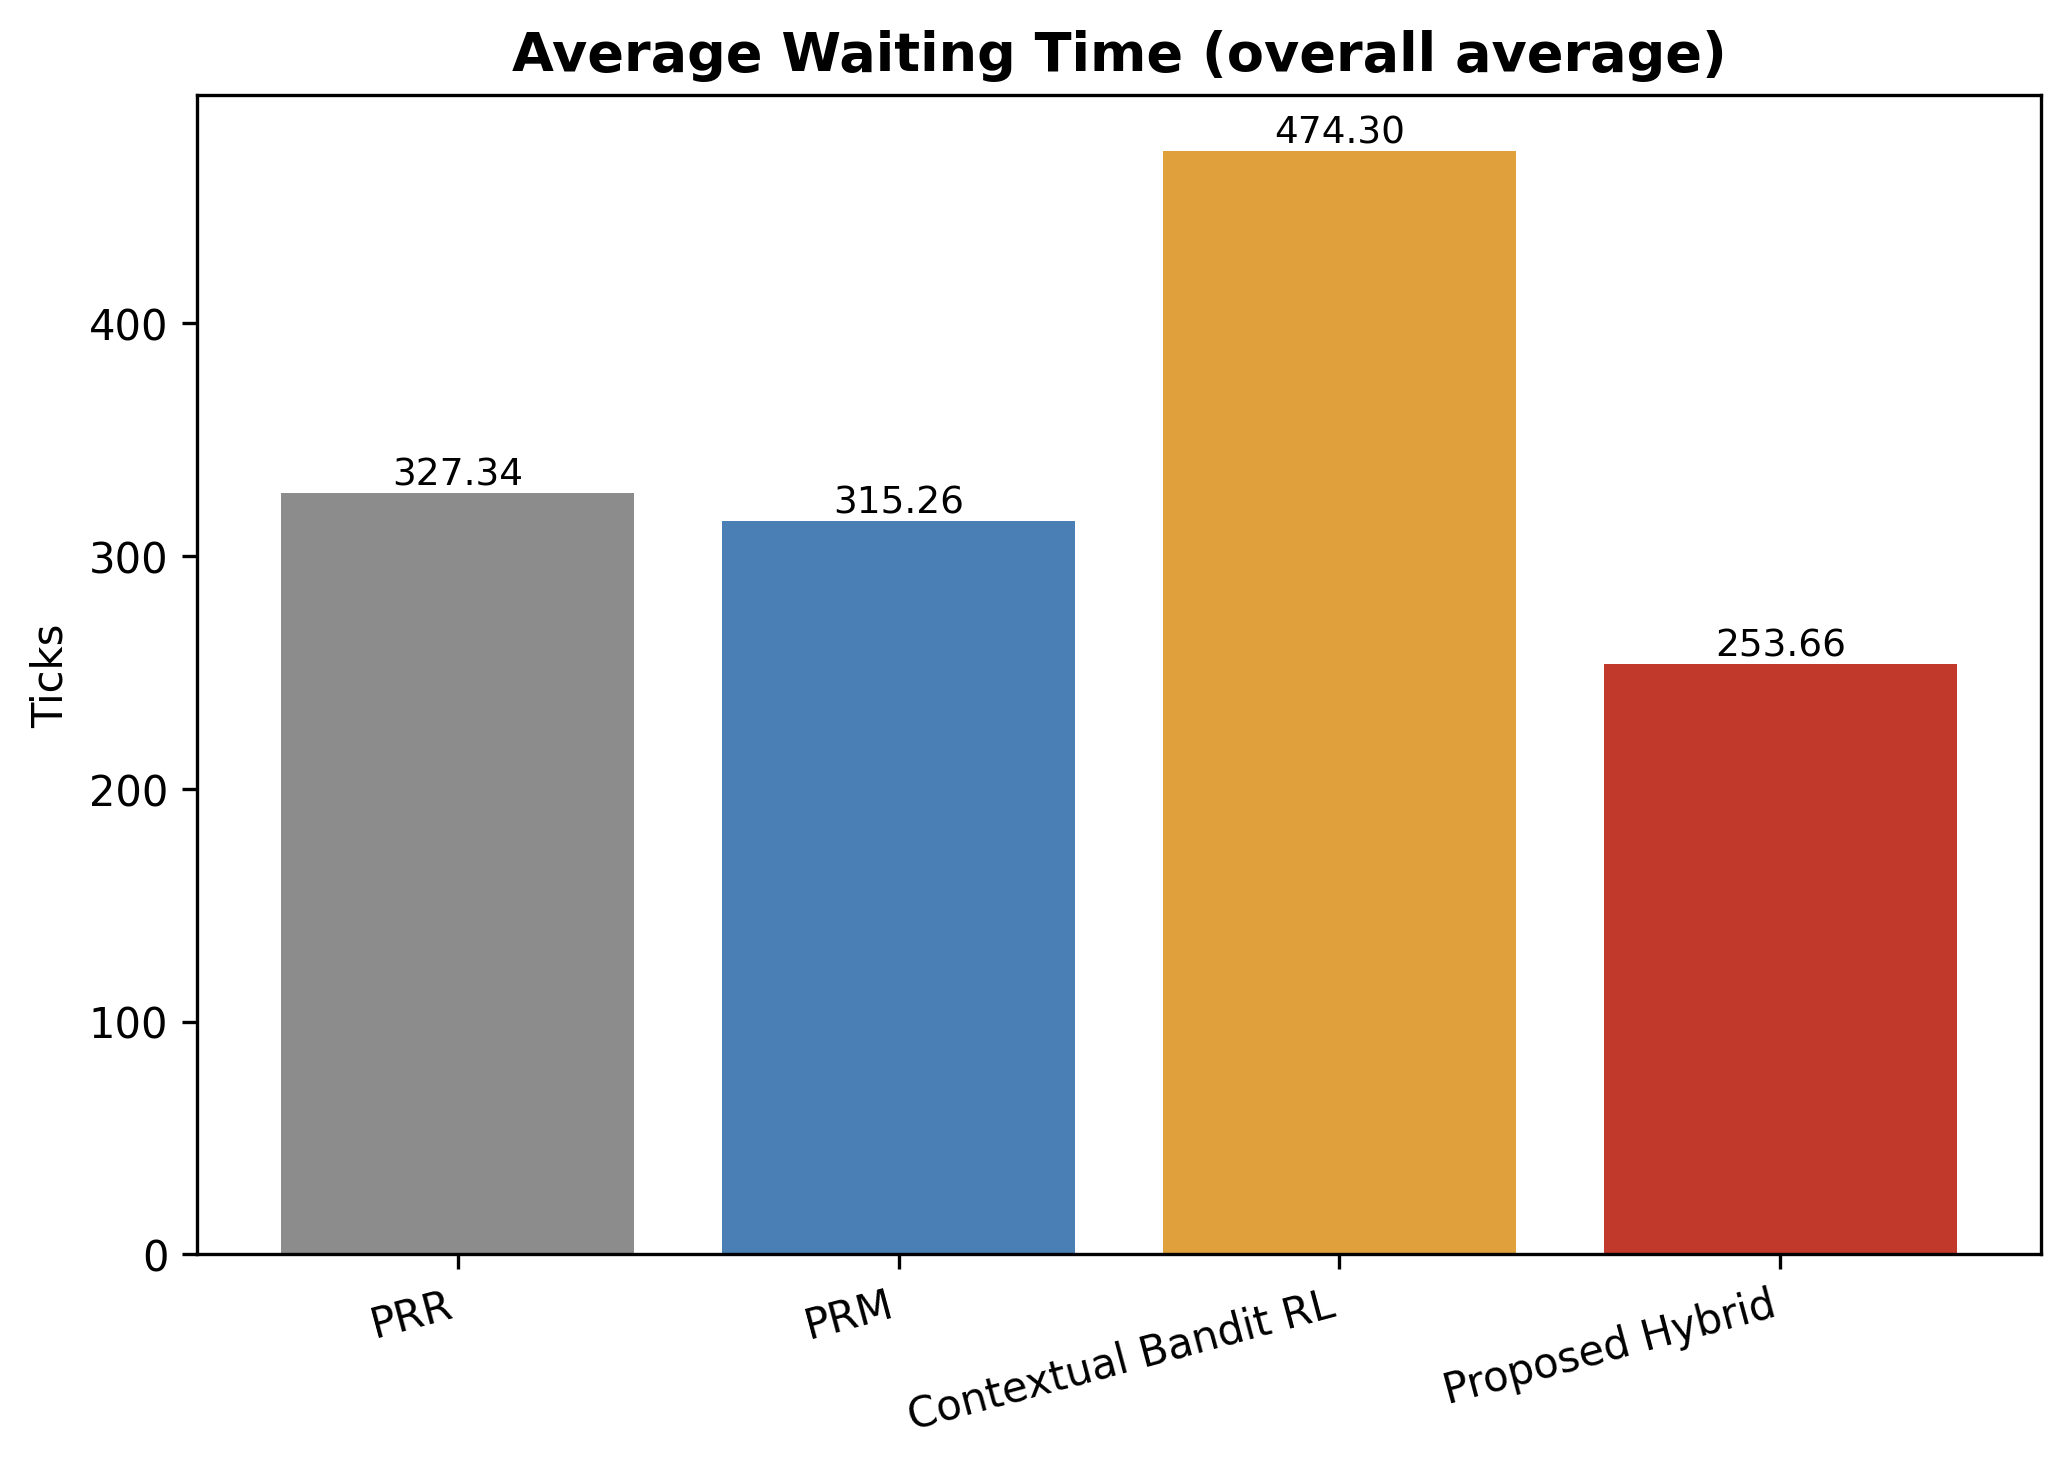
\includegraphics[width=\columnwidth]{results/avg_waiting_time.png}
\caption{Overall waiting-time comparison across evaluated scheduling policies.}
\label{fig:baseline}
\end{figure}

\begin{figure}[htbp]
\centering
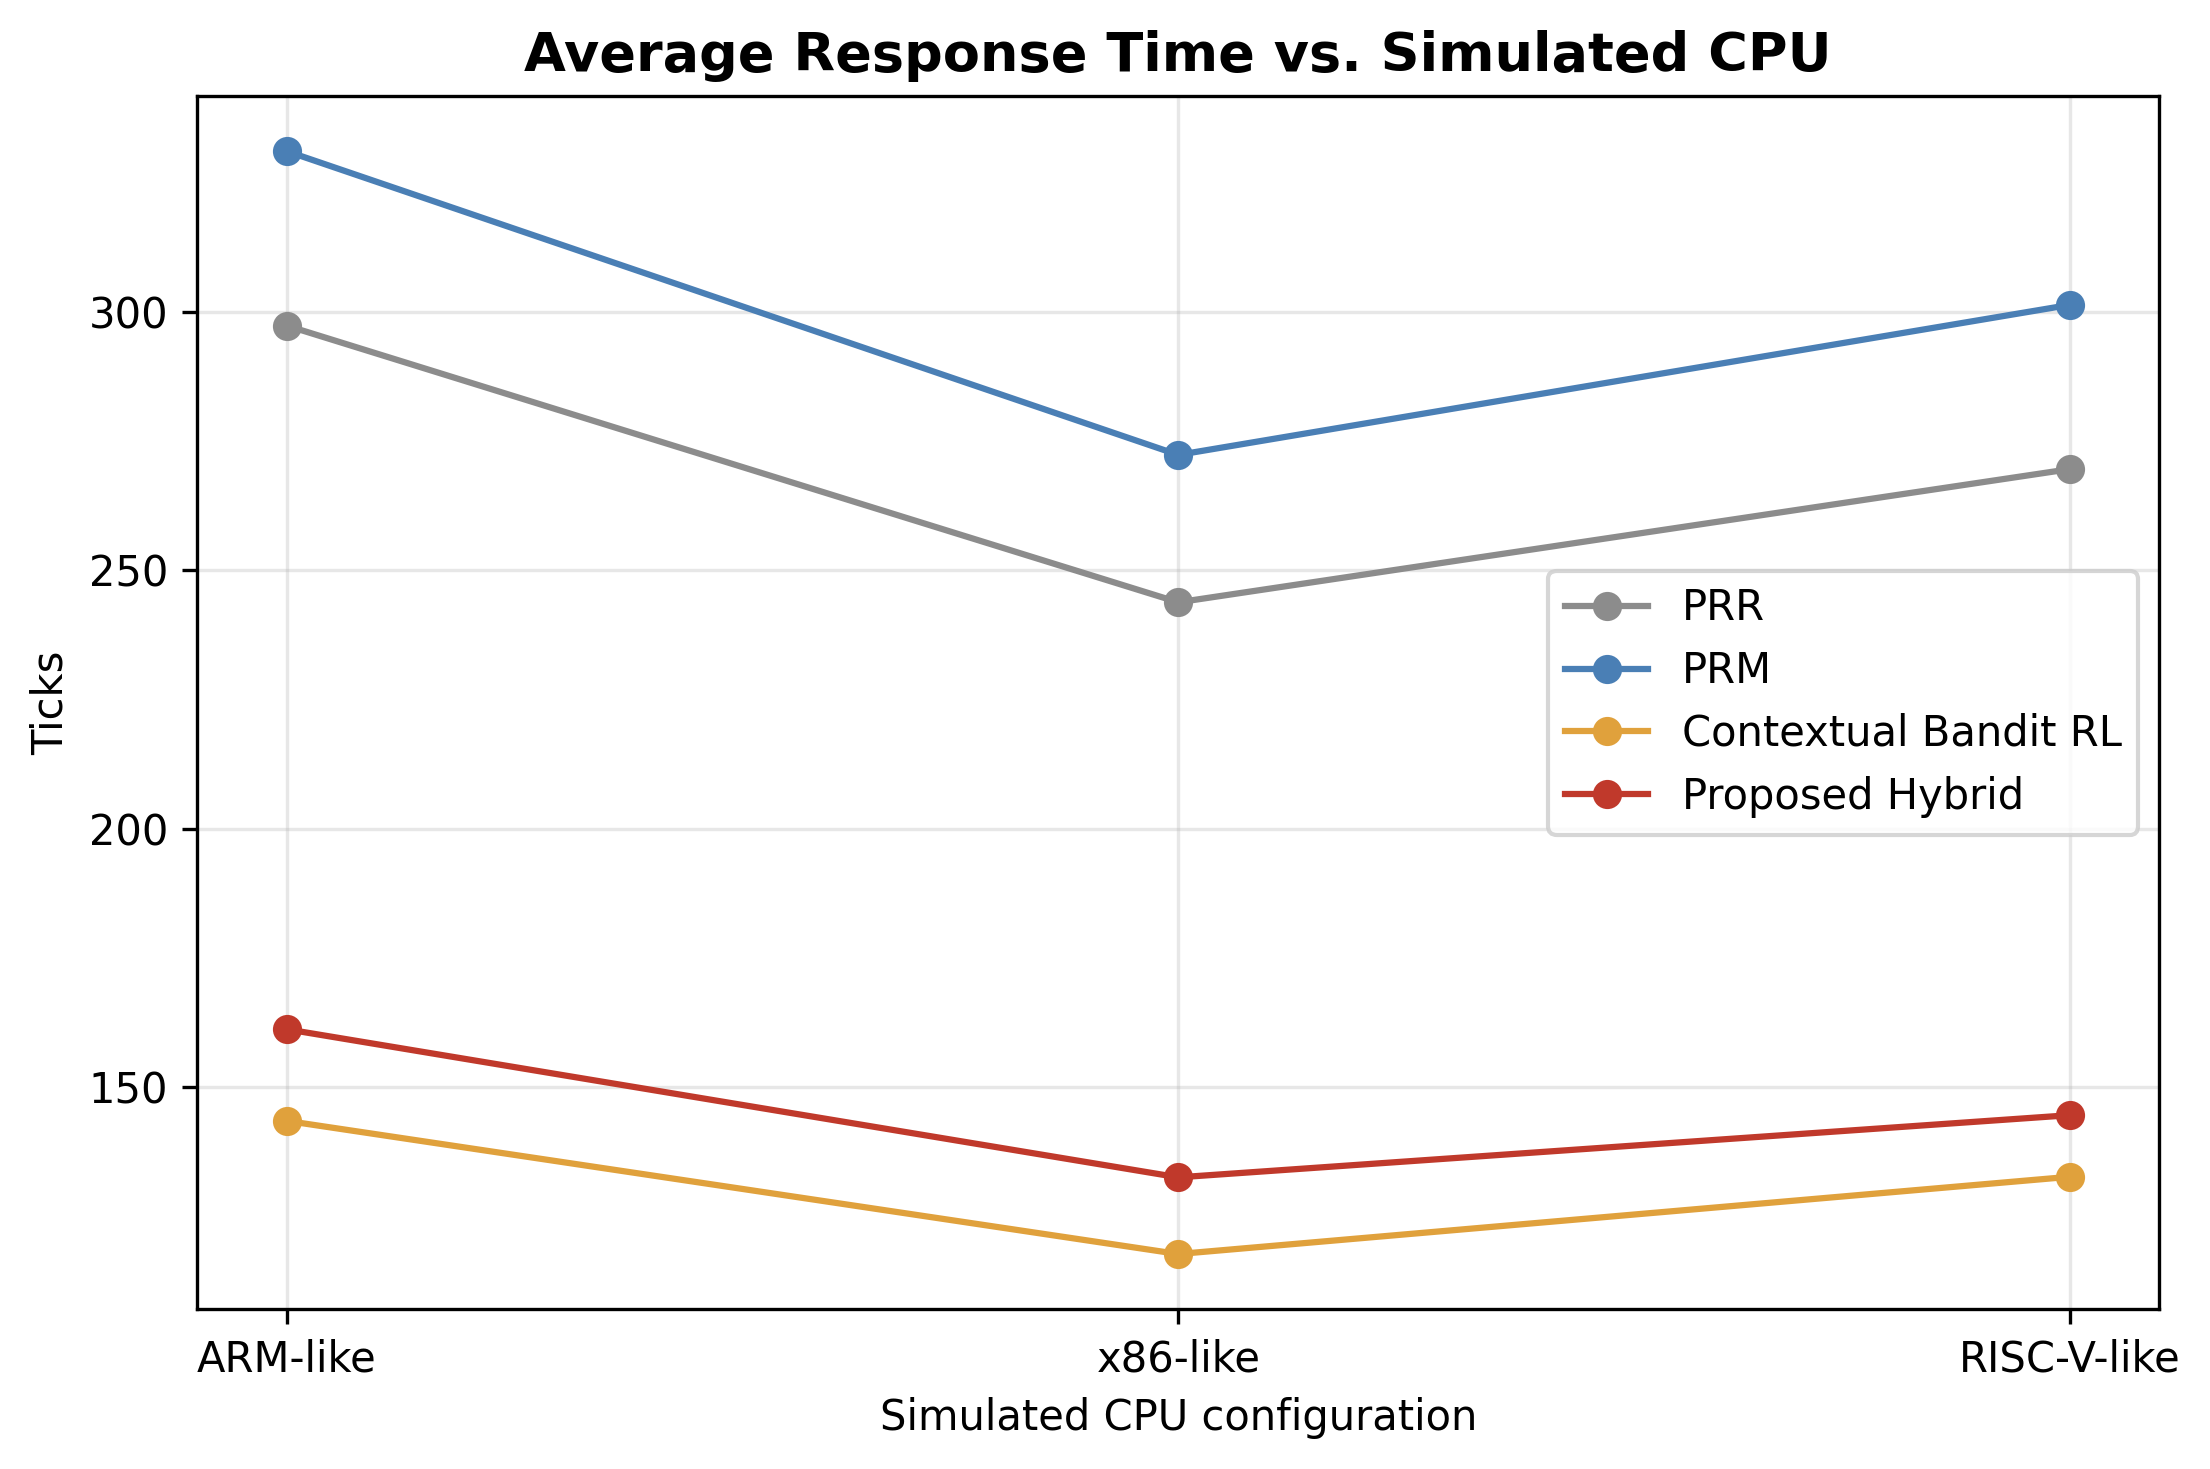
\includegraphics[width=\columnwidth]{results/avg_response_time_vs_cpu.png}
\caption{CPU-aware response time across ARM-like, RISC-V-like, and x86-like simulated configurations.}
\label{fig:cpu_aware}
\end{figure}

\subsection{Cross-Architecture Evaluation}
The multi-platform evaluation extends across 1,500 scheduler runs by modulating architectural speed and power factors. As detailed in Table \ref{tab:cpu_results}, the Proposed Hybrid scheduler consistently establishes the lowest waiting times across all simulated CPU configurations: \textbf{279.46 ticks} for ARM-like, \textbf{252.98 ticks} for RISC-V-like, and \textbf{228.55 ticks} for x86-like, while its bounded first-touch boost preserves response-time gains without excess switching.

\begin{table}[htbp]
\caption{CPU-Aware Waiting and Response Results (1,500 Runs)}
\begin{center}
\begin{tabular}{llrr}
\toprule
\textbf{CPU Configuration} & \textbf{Scheduler} & \textbf{Wait Time} & \textbf{Response Time} \\
\midrule
ARM-like & PRM & 346.55 & 331.16 \\
& PRR & 359.49 & 297.38 \\
& CB-RL & 520.60 & 143.39 \\
& \textbf{Hybrid} & \textbf{279.46} & \textbf{161.13} \\
\midrule
RISC-V-like & PRM & 315.15 & 301.40 \\
& PRR & 327.32 & 269.59 \\
& CB-RL & 479.00 & 132.57 \\
& \textbf{Hybrid} & \textbf{252.98} & \textbf{144.50} \\
\midrule
x86-like & PRM & 284.06 & 272.34 \\
& PRR & 295.21 & 243.80 \\
& CB-RL & 423.30 & 117.61 \\
& \textbf{Hybrid} & \textbf{228.55} & \textbf{132.46} \\
\bottomrule
\end{tabular}
\label{tab:cpu_results}
\end{center}
\end{table}

\begin{figure}[htbp]
\centering
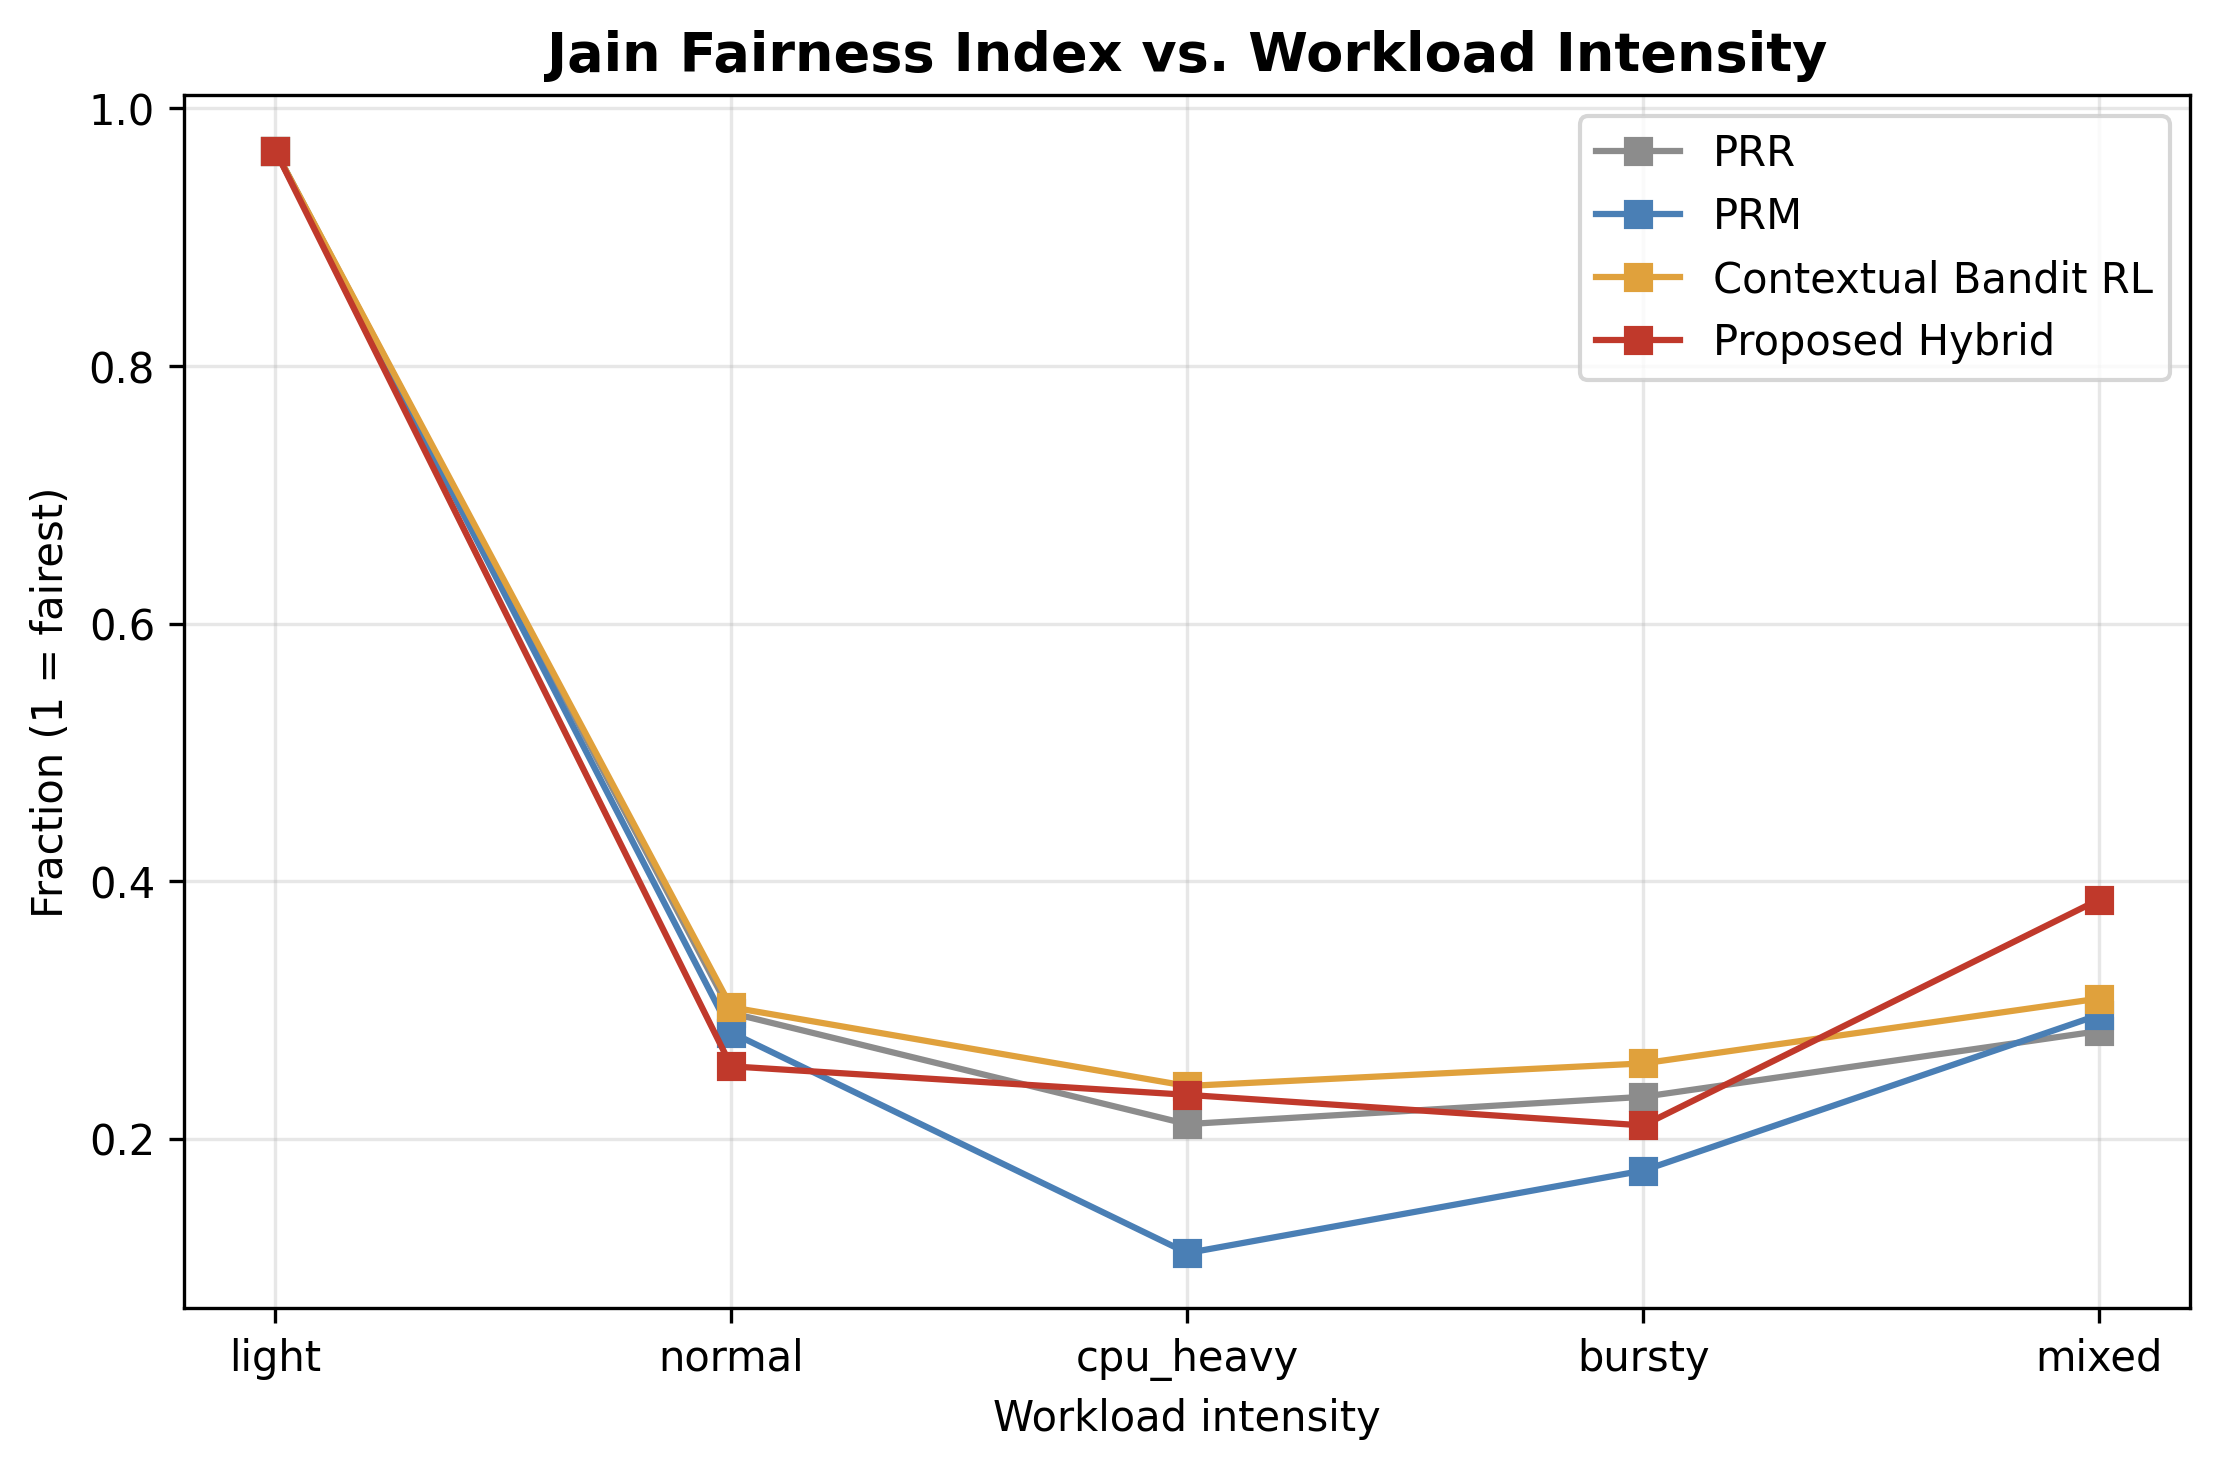
\includegraphics[width=\columnwidth]{results/fairness_jain_index_vs_workload.png}
\caption{Jain fairness index across workload profiles, demonstrating Hybrid competitiveness under bursty conditions.}
\label{fig:fairness}
\end{figure}

\begin{table}[htbp]
\caption{CPU Sanity Verification (5 VMs, Seed 1)}
\begin{center}
\begin{tabular}{lrrr}
\toprule
\textbf{CPU Model} & \textbf{Sim. Duration} & \textbf{Wait Time} & \textbf{Throughput} \\
\midrule
ARM-like & 91.788 & 35.334 & 0.05447 \\
RISC-V-like & 85.190 & 33.481 & 0.05869 \\
x86-like & 78.780 & 30.234 & 0.06347 \\
\bottomrule
\end{tabular}
\label{tab:sanity}
\end{center}
\end{table}

\section{Discussion and Limitations}
The empirical evaluation indicates that bounded first-touch prioritization avoids the excessive churn of unconditional first-touch dispatch. The Hyper-Optimized Hybrid policy minimizes waiting and turnaround among the tested x86-like policies, improves deadline adherence over PRM, and reduces context switching below Turbo V4. Context-switch reduction directly curtails dispatching latency, making the policy suitable for resource-constrained edge virtualization.

Current limitations include reliance on single-core discrete event simulation and synthetic power proxies rather than physical instrumentation. Subsequent research will address multicore migration, DVFS hardware coupling, and real-time hypervisor integration.

\section{Conclusion}
This study presented a context-aware hybrid reinforcement learning framework for CPU scheduling in lightweight virtualized systems. By augmenting contextual bandit learning with online workload prediction, nonlinear aging, density-aware completion hysteresis, hyperbolic SRTF bias, and a bounded first-touch score boost, the Hyper-Optimized Hybrid scheduler delivers \textbf{132.46}-tick response time on the x86-like benchmark, \textbf{228.55}-tick waiting time, \textbf{0.4171} fairness, \textbf{0.5561} deadline-miss rate, and \textbf{71.56} context switches. These results improve both waiting time and context switching over Turbo V4.

\begin{thebibliography}{00}
\bibitem{b1} W. Cui, C. Wang, Q. Yu, C. Wei, and R. Zhang, ``Optimizing CPU scheduling and inter-VM communication for lightweight virtualization using reinforcement learning,'' \textit{Future Generation Computer Systems}, vol. 185, Art. no. 108612, 2026, doi: 10.1016/j.future.2026.108612.
\bibitem{b2} T. Zhou and M. Lin, ``CPU frequency scheduling of real-time applications on embedded devices with temporal encoding-based deep reinforcement learning,'' \textit{Journal of Systems Architecture}, vol. 142, Art. no. 102955, 2023, doi: 10.1016/j.sysarc.2023.102955.
\bibitem{b3} P. Li, Y. Xiao, J. Yan, X. Li, and X. Wang, ``Reinforcement Learning for Adaptive Resource Scheduling in Complex System Environments,'' \textit{arXiv:2411.05346}, 2024, doi: 10.48550/arXiv.2411.05346.
\bibitem{b4} X. Sun, Y. Duan, Y. Deng, F. Guo, G. Cai, and Y. Peng, ``Dynamic Operating System Scheduling Using Double DQN: A Reinforcement Learning Approach to Task Optimization,'' \textit{arXiv:2503.23659}, 2025, doi: 10.48550/arXiv.2503.23659.
\bibitem{b5} D. R. Rinku and M. AshaRani, ``Reinforcement learning based multi core scheduling (RLBMCS) for real time systems,'' \textit{International Journal of Electrical and Computer Engineering}, vol. 10, no. 2, pp. 1805--1813, 2020.
\bibitem{b6} G. Perin, F. Meneghello, R. Carli, L. Schenato, and M. Rossi, ``EASE: Energy-Aware Job Scheduling for Vehicular Edge Networks With Renewable Energy Resources,'' \textit{IEEE Transactions on Green Communications and Networking}, vol. 7, no. 1, pp. 339--353, 2023.
\bibitem{b7} Y. Zhang, X. Zhao, Z. Li, J. Yin, L. Zhang, and Z. Chen, ``Integrating Artificial Intelligence into Operating Systems: A Comprehensive Survey on Techniques, Applications, and Future Directions,'' \textit{arXiv:2407.14567}, 2024.
\end{thebibliography}

\end{document}
